\chapter{Theoretical Approach}
\label{cha:theoreticalapproach}

Once a decision is made in favor of a project using a static site generator, first challenges may already arise:

\begin{itemize}
  \item What kind of media is being used? Images, videos, or just text?
  \item How is the project structured? How many independent permalink structures are there?
  \item How many content authors are there? How often is content added or altered?
  \item How steady is the site design? Does the site have more than one independent design flow?
\end{itemize}
Some content-related issues may not be improved in a predictable amount of time, but even in projects where only a high amount of content productivity is pursued, developers are forced to keep the build pipeline performant and responsive to the content author's needs.

\section{Challenges}
\label{sec:challenges}

As already stated above in the introduction, nearly every web project bears challenges to solve, both for developers on the one hand, and for content creators on the other hand. While content creators mostly need to solve structural issues in the published content, developers are mainly responsible for supporting authors in technical questions, as well as constantly keeping an eye on the backend development. This might go from always keeping the underlying modules updated, to populating the source code with design or template changes, to finally maintaining the build pipeline and deployment setup.

\subsection{Distributed development}
\label{sec:challenges-distributeddevelopment}

When it comes to administer a static site project, it is very likely, that there will not be any possiblity of working on the same project in the same environment in a linear way. Instead, every developer will have to have a local install of the used generator at his/her disposal, together with access to a remote repository of a version control system for exchanging the current development process with other project maintainers. The main reason for that is the fact, that unlike content authors, developers do have the obligation of installing or maintaining the project's dependencies \cite[85]{dhillon2016}, thus not only for testing reasons.

If using GitHub for example, content editors, on the other hand, may easily make use of the built-in ``In-Page Code Editor'' (see Fig. \ref{fig:github-page-editor} on p. \pageref{fig:github-page-editor}), which also provides an optimistically rendered version of the current content, although without making use of the project's style sheet.

%% Graphic of separating project repositories
\begin{figure} % h-ere, t-op, b-ottom, p-age
    \centering
    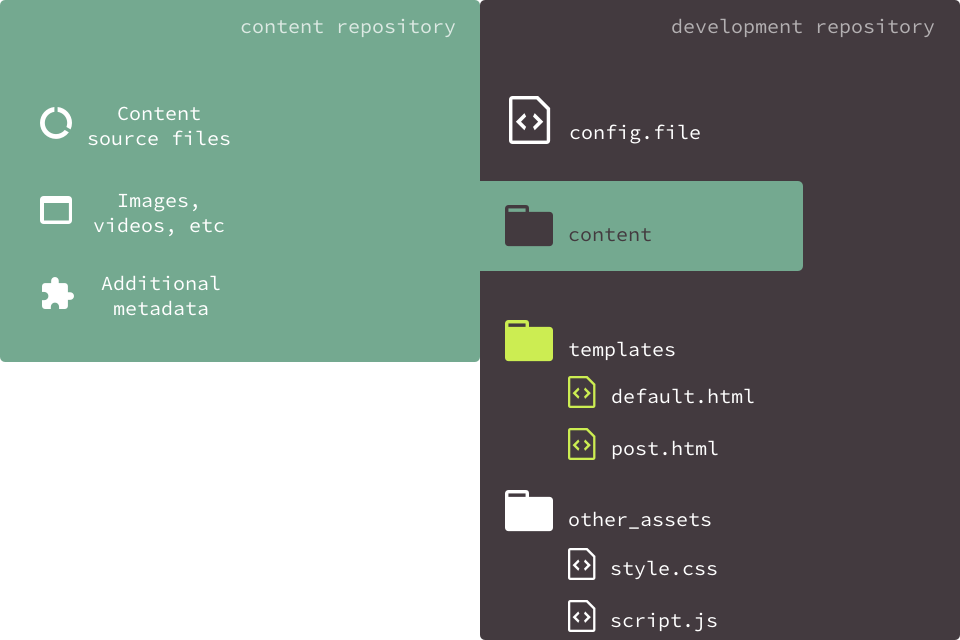
\includegraphics[width=0.9\textwidth]{challenges-repositories.png}
    \caption{A graphic showing the stylized separation of a project into a \emph{content} and a \emph{development} repository. The content authors may only be granted access to the content repository, while developers should be granted access to both, thus providing a seamless integration for the content into the build pipeline flow (see Fig. \ref{fig:build-pipeline} on p. \pageref{fig:build-pipeline}).}
    \label{fig:repository-separation}
\end{figure}
%

\subsubsection{Separating content from code}
As constantly growing static site projects may sooner or later come to a point, where content progression differs from development progression, it might be useful to separate both parts into independent repositories (see Fig. \ref{fig:repository-separation}). This especially makes sense, if the content editor team is also separated from the development team and therefore an additional level of security against accidental branch intermixture is needed.

\subsubsection{Merging only using pull requests}
However, if this kind of strong division is not desired anyhow, another option would be to limit access to the development repository in a way, that everyone may \emph{fork} a repository, but only certain project users are allowed to \emph{merge} external branches into the main development tree. On GitHub, \emph{pull requests} may be used. These pull requests allow any user to announce his/her contribution to the project using a commit history of a forked repository. The source project owners may then decide whether or not to merge the announced changes and also have the chance to express their point of view via comments directly on the pull request to its creator \cite[p. 394f]{loeliger2012version}.

The point in time a pull request is created is although subsidiary, as further development on the specific branch is as well automatically included, as per-line comments are also removed, once the specific line of code has been modified in a following commit \cite{GithubPullRequests}. Furthermore, the possibility to merge is checked after every commit pushed to the respective branch, so the responsible users always know, if a merge operation may be successfully executed before being able to complete the process by clicking the green ``Merge pull request'' button. Otherwise, a merge is only possible after locally checking out the pull request and processing it via the command line \cite{GithubMergePullRequests}.

\subsubsection{Staging versions}
Working with separate remote branches on a version control system like Git also allows for staging environments and therefore testing out different versions of the projects concurrently. The public version however, visible to all clients visiting the website, remains the most stable and might receive only well-tested or well-considered updates as the very last step in the ongoing development.

To achieve this goal, a testbed is necessary and may be realized using another branch besides ``master''. Sometimes an additional ``bleeding edge'' version is also likely to be included in the build process. Based on this strategy, it is easy to control and maintain different revisions at the same time and nevertheless infer the functionality of different proof of concepts for merging them into the public version later on.


\subsection{Build cycle completion}
\label{sec:challenges-buildcyclecompletion}

One of the major challenges remains the issue of providing a ``real website look and feel'' to the content editor. Whereas authors in dynamic CMSs are presented with an already pre-rendered version of the newly added content (since the underlying system is not dependent on any template rendering before deployment), static site generators first offer a glance of the author's work, after the whole build pipeline process succeeded in its render flow, unless other pre-caching methods are used. Yet, most static site generators do not include such kind of tools by default.

Based on the size and the amount of files in the website source code, this time frame can easily grow linearly. If there are also additional tasks added to the build process, such as resizing images to different screen sizes for providing a  responsive user experience, the computational effort may easily get out of hand and therefore the duration until the content editor first sees the result of his/her work simply gets unacceptable.

\subsubsection{Possible problems of long-lasting build processes}
Waiting for the completion of the build pipeline can cause severe recesses in the work performance of a content editor or developer, as mostly any further work depends on its success, while a failure is often combined with time loss beforehand and intensive bug hunting afterwards -- probably resulting in even more consecutive build pipeline failures. This assertion may not only be linked to crucial modifications in development, also the smallest hotfixes might as well provoke a full rebuild without justifying the whole effort.

Furthermore, being forced to wait in line as a developer may cause him-/herself to loose track on the development process, thus the introduction of sustainable bugs (although not resulting in a build failure) is more likely. Additionally, mindlessly executing build cycles may even lead to data loss or blocking the workflow of other contributors.

%% Graphic of caching theory
\begin{figure} % h-ere, t-op, b-ottom, p-age
    \centering
    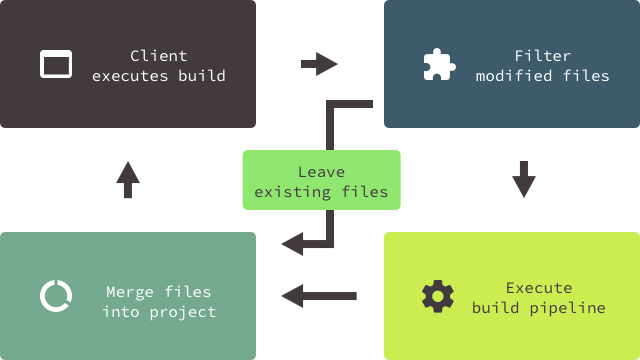
\includegraphics[width=0.9\textwidth]{challenges-caching.png}
    \caption{A graphic showing the theoretical approach of a build process flow, supported by caching.\\
    After the \emph{client} (content creator, developer) executes a build, the included caching mechanism should filter modified or added files and send them to the build pipeline. After the build succeeded, the newly built files should be merged with the already existing files to form an updated version of the website root.}
    \label{fig:caching}
\end{figure}
%

\subsubsection{Choosing an appropriate caching method}
Speeding up a build process can be done via \emph{caching}. The right caching method should differ between unmodified content and files which actually have been reworked or were newly introduced into the project source. Using this sort of information, the algorithm might only choose the latter files, send them to the build pipeline and assemble the outcome to the already existing project build (see Fig. \ref{fig:caching}).

Although a few static site generators already include some sort of caching methods -- although most of them only work locally (like Hexo's Warehouse, see ch. \ref{sec:hexo-technology}), a first step is made. It should significantly improve the build duration for local development, as long as the optimal cache storage is being used. Hexo's Warehouse uses a \emph{JSON} file as persistant storage, while the temporary storage lies in the Computer's RAM. This is fine for smaller projects, but could also lead to critical memory issues when used in projects containing a huge amount of files. For bigger data sets, it would be possible to use caching in conjunction with databases like \emph{SQLite} using the \emph{JSON1} extension\footnote{\url{https://www.sqlite.org/json1.html} -- JSON1 documentation on SQLite's website.}, however, the necessary effort at the beginning for providing a working mechanism should be well considered.

Nevertheless, a major issue still remains, as the local cache may not easily be transferred to other contributors or deployment engines, so that the first build after each pull does not take advantage of any speed up technique. Moreover, the methods mentioned above all use a significant amount of computing power to provide a useable cache, which could lead to problems and unwanted slowdowns on portable devices.

\subsubsection{Determination of cacheable contents}
When having overcome the decision and setup of the respective caching system, the next step would be to select cacheable files, as not every file has the same impact on the project source. While normal blog posts mostly belong to their own, unless there is probably a preview featured somewhere, a template file on the other hand, is often a dependency for many blog posts. Therefore, it can be said, that a working cache is more important for a commit only containing blog posts, than for a commit which only contains template files.

%% blargh -- dependency management, sitemap, etc...

\section{Solution strategies}
\label{sec:solution-strategies}

A primary task would be the focusing on critical issues to at least boosting the project's overall performance noticeably without losing too much track. This may be worked on in terms of collaboration, as well as in the project's setup, where on the one hand the team's performance and on the other hand the build engine's performance should be improved.

A lot of issues can be covered using GitHub's API, although some project specific adaptions are still necessary. Nevertheless, the API provides enough information for quickly perceiving a sufficient overview of the respective repository.


\subsection{Distributed development on GitHub}
\label{sec:solutions-distributeddevelopment}

Based on GitHub's API and the advantages of using Git as version control system, it is definitely a significant benefit to equip all project contributors with a GitHub account. While the public, open-source model is free of charge (see Sec. \ref{sec:github-history}), there are also different pricing models offered for privately held projects, which should be hidden to the public\footnote{\url{https://github.com/pricing} -- GitHub's pricing models.}.

Although dependent on financial expenditures, the additional value of working on a project with closed source (though it may be released as open source somewhere in the future) may be worth considering. Yet, full-featured access to the API is also included in the free tier though.

Not only GitHub offers a queryable API, also \emph{Bitbucket} provides an API with similar response data\footnote{\url{https://developer.atlassian.com/bitbucket/api/2/reference/} -- Bitbucket's API documentation.}, although certain features are missing, compared to GitHub. These missing features include for example certain project download functions, among others.

In addition to the API, GitHub's built-in In-Page Code Editor plays an important role for choosing it as core support tool for this project. Therefore, merging using pull requests and a continuous branching model for supporting staging versions qualify as proposed strategies to developers.


\subsection{Build cycles}
\label{sec:solutions-remotebuilding}

Supporting content authors in their workflow also means to not require them to install unnecessary build tools manually, unless critically needed. Due to the possibility of using GitHub's In-Page Editor, the whole Git checkout, commit and push process becomes in a way redundant too. Moreover, the online editor automatically creates pull requests on demand, so that the respective project owners should get notified automatically, if a merge is possible and therefore an update of the currently published project may be initiated.

Normally, a responsible user would pull the new state after a merge of the pull request, then execute the build pipeline. After the build process succeeded, he/she then has to take care for updating the webroot on the server, so that the newest version of the website gets delivered to the client upon request. However, this practice may easily get cumbersome, as the respective developer might get distracted by checking out new branches and possibly leaving behind his/her own work for the moment. Moreover, if the deployment has to be done manually, additional mistakes may happen during the whole action.

In this case, it makes sense to remotely outsource the build service and to possibly even automatically execute the render cycle. Used in conjunction with GitHub's \emph{Webhooks}, an external service would receive a build execution order via a HTTP POST request, based on certain predefined events in the GitHub repository \cite{GithubWebhooks}. Apart from the information the webhook provides, the service would even accept custom build options issued by responsible users, as the endpoint has to be publicly available anyhow. Once a build succeeds, the service should then notify a predefined list of users about the render cycle result and provide the outcome via download possibility.

\subsubsection{Existing remote services for static site generators}
\emph{CloudCannon}\footnote{\url{http://cloudcannon.com} -- CloudCannon, the Cloud CMS for Jekyll.} is probably the most popular online static site generator and offers a commercial external building service for Jekyll projects, together with source access using a GitHub or Bitbucket repository. According to its documentation, it currently supports Jekyll projects running v2.4.0 or newer\footnote{\url{https://docs.cloudcannon.com/building/versions/} -- Supported versions on CloudCannon documentation.}. It features a project file explorer and presents every new project as opinionated as Jekyll usually does (see Sec. \ref{sec:jekyll-technology}), as well as an automatic deployment service on their own subdomains. However, access to the rendered website files is not included, so every customer is dependent on using their hosting service.

\emph{BowTie}\footnote{\url{https://bowtie.io} -- Website of BowTie.} is similar to CloudCannon and is also offering a commercial online service. It seems to be a much more standalone service than CloudCannon, though it also offers GitHub integration, as well as custom Webhooks for event-based actions on external services.

%% Screenshot of Pancake push fail
\begin{figure} % h-ere, t-op, b-ottom, p-age
    \centering
    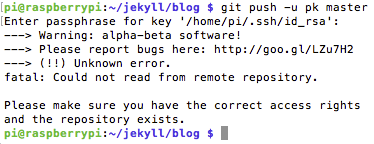
\includegraphics[width=0.75\textwidth]{remote-pancake.png}
    \caption{A screenshot of an approach to pushing a Jekyll project to \emph{Pancake}. As a result, the operation failed with an ``Unknown error''.}
    \label{fig:remote-pancake}
\end{figure}
%
\emph{Pancake}\footnote{\url{https://www.pancake.io} -- Website of Pancake.} is a free service for externally building static sites. It features an engine auto-detection and currently supports \emph{Jekyll, Wintersmith, Pelican, Sphinx, Hyde} and \emph{Middleman}\footnote{\url{https://github.com/pancakeio/detect/blob/master/heuristics.go} -- Currently supported static site generators by Pancake in raw source file on GitHub.}. Due to its non-commercial version, several restrictions are to be considered \cite{PancakeGitProjects}.

However, the service does currently not run stable, as an initial project setup failed (see Fig. \ref{fig:remote-pancake}). It seems that Pancake uses a post-receive hook for automatically trying to build a project, once it detected the underlying engine type. This causes waiting time for the developer on the one hand, but on the other hand informs whether a build was successful or failed. During another push attempt, it failed, as \emph{bundler}\footnote{\url{http://bundler.io} -- Bundler, a gem dependency manager.}, a gem dependency management tool required by Jekyll, was not mentioned in the ``Gemfile'' contained in the repository.

\subsection{Caching}
\label{sec:solutions-caching}

As stated before, most static site generators do not contain any form of caching mechanism by default -- if they do, caching is limited to the local machine a build is executed on. Since there is probably not an easy way of providing a form of remote caching, as this largely includes the necessity of external services to exchange a common status, as well as an index containing information about source and destination files for later rebuilds, it needs an equivalent strategy, which merely contains these information from a certain point in the past to the present, without relying on physical file structures to be exchanged.

Furthermore, such a caching strategy must be universally useable across all operating systems and ideally does not require any additional setup from the user. Moreover, it should also feature hassle-free integration into any project without depending on an external, yet unused service.

Keeping all of these issues under consideration, not every suggestion might get featured equally in the final solution -- the main reason is, that a kind of transformation like the one caused by a build pipeline always needs an existing status to build up from. So, tradeoffs are likely to accompany any form of decision to be made in this case.

\subsubsection{Caching based on diff}
As Git was chosen as version control system, diff is already part of the development suite. Therefore, a gapless detection of development progress between two arbitrary commits is possible. The diff format can be parsed to JSON and makes it easy for use in JavaScript. Thus, its usability for further processing on application level is assured\footnote{\url{https://runkit.com/saschazar21/diff-parsing-demo} -- An interactive example for fetching and parsing a diff-file.}.

The most important parts of a diff representation in this context are the file paths, as well as the type of modification on each file affected in the respective time span. Considering this kind of information, an existing repository might be quickly divided into unaffected and affected files -- where affected files, as well as their dependents possibly need to be selected for a rebuild. The final decision of the rebuild extent based on the diff, however, should be based on heuristics.

To conclude the consideration of using diff, the approach explained above is different from ``classical'' caching. Such a mechanism, founded on diff, is not dependent on support-files produced on its own (like a caching catalogue), but it requires a consistent and strict git workflow, otherwise it has no control over untracked files.

\section{Preparing for implementation}
\label{sec:primarythoughts}

After looking at challenges and possible solutions to them, a few keywords are essential:

\begin{description}
  \item[Remote] -- Outsorce long-lasting actions to an external service.
  \item[Cache] -- Speed up builds by making use of already finished work.
  \item[Versioning] -- Keep track on development and possibly revert, if necessary.
  \item[Branches] -- Let different parts of development evolve to their own speed.
\end{description}

While it may appear, that the above list is too fixated on version control systems, it should be clear now, that especially Git qualifies core companion to any website project, especially when the project itself is maintained by multiple developers, designers and/or authors. Being aware of GitHub as social code management tool and moreover the benefits of its API, the foundation stone should be laid (see ch. \ref{sec:solutions-distributeddevelopment} on p. \pageref{sec:solutions-distributeddevelopment}).

%% Graphic of basic api flow
\begin{figure} % h-ere, t-op, b-ottom, p-age
    \centering
    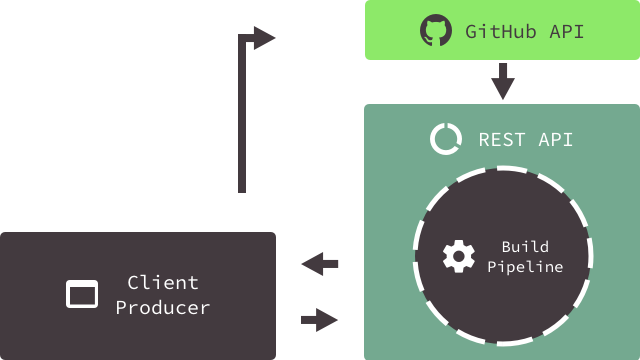
\includegraphics[width=0.75\textwidth]{api_flow.png}
    \caption{An abstract flow visualization of the planned request cycle. The client (developer, content creator) manages his/her code on GitHub. Based on the respective configuration, a build cycle may be triggered either using a GitHub webhook, or by manually sending a POST request to a certain endpoint.    That request then gets caught by the REST API, which creates an instance of the build pipeline. The pipeline requests data of the project from GitHub and sets up the project configuration. After a successful build, the REST API provides a downloadable archive of the newly built webroot.}
    \label{fig:api-flow}
\end{figure}
%

Since the tool should also be remotely accessible, it makes sense to also design it as RESTful API, for handling programmatical access as well as access from possible frontend apps lying on top. Furthermore, its main work cycle might get detached for neither distracting users due to ordering them to wait until it finished, nor blocking access in between (see Fig. \ref{fig:api-flow}).

However, the most important part behind these thoughts is the choice of the ideal static site generator.


\subsection{Choosing a static site generator}
\label{sec:primarythoughts-generator}

Due to the fact, that the choice of the best possible static site generator is the linchpin for a project like this, the evaluation needs to cover its usability, pluggability, customizability and overall maintenance, as well as the level of its general support. First and foremost, the installation process should be as easy as possible and not rely on too many third-party dependencies, which are probably not needed afterwards. Through this, it may be guaranteed, that also users, who are foreign to development, are likely to set up an instance on their local machines, although not critically required. This creates awareness for the project structure and therefore may lead to less support requests in the future.

The programming language of the chosen static site generator does have to be considered well, as it has to fit seamlessly into a planned REST API, in the best case without any further adapter in between. This should make it also easy to hook additional code into the configuration step, if needed. Ideally, it emits events as well, so any host process knows when a detached process is finished.

All in all, the best possible solution seems to be \emph{Metalsmith} (see ch. \ref{sec:metalsmith} on p. \pageref{sec:metalsmith}), as it not only offers a pluggable module ecosystem, but also access to a JavaScript API, among others. Together with some custom tweaks (e.g. dynamic module loading), an independent build setup for each project may be injected using only a specific configuration file.


\subsection{Constructing a REST API}
\label{sec:primarythoughts-restapi}

JavaScript proved its universality due to its usage both on client- and server-side, thus, a major advantage is its common knowledge among developers combined with a low barrier to entry for people, which are already found in frontend-development.

Node.js is a server-side implementation for JavaScript, backed by Google's V8 engine, which directly translates the scripting language into machine code \cite[4]{cantelon2017node}. This perfetly supports developers in reducing their tradeoff for possibly having to handle multiple ecosystems at once. A seamless integration of Metalsmith into the API service may therefore happen without much hassle.

The easy installation is supported by several third-party apps like Node Version Manager (\emph{NVM})\footnote{\url{https://github.com/creationix/nvm} -- NVM's repository on GitHub.} and mostly will not need any admin rights, which makes it ideal to use on hosting environments without root access (unlike PHP or Ruby for example). Although not equally well supported among the most popular operating systems, at least MacOS and Linux provide a stable enough environment for NVM.

Looking for a framework for setting up an API, \emph{Express}\footnote{\url{http://expressjs.com/} -- Website of Express.} seems to be the perfect fit, as it consists only of a very basic setup -- similar to Metalsmith -- but may be easily enhanced using different node modules, thus providing a uniquely shaped web application in contrast to conventional, monolithic frameworks like \emph{Django} or \emph{Ruby on Rails} \cite[176]{cantelon2017node}.

% Express sample basic configuration
\lstinputlisting[caption={An example for a basic express.js setup, roughly taken from \url{http://expressjs.com/en/starter/hello-world.html}.\\
In this case, a web application listens for a \emph{GET} request on its root path ``/'' and responds with a ``Hello World!'' message.}, label={list:express-setup}, language=JavaScript]{chapters/04-theoretical-approach/_support/express.js}

As a result, the main purpose of such an express application would be acting as a web-based infrastructure for the underlying build pipeline. Based on different REST endpoints, as well as their request parameters, executing a uniquely configured Metalsmith process on a project directory within the API's file tree should be possible without any further external interaction requirement. The project directory would be provided using an appropriate GitHub repository, requiring only a basic, as little opinionated configuration as possible, together with a public access possibility to the repo.

Additionally, to benefit most from any remote outsourcing, a current production-ready version of the project may be held available at a special endpoint for downloading at any time. In this case, further processing is enabled without waiting for completion of any build cycle beforehand, unless the source code received any updates through development.


\subsection{Selective rendering}
\label{sec:primarythoughts-rendering}

While the theoretical foundations for a project covering the use case of static site generation are now defined, a constantly growing amount of necessary build time still remains as one of the core problems. Caching across remote machines is likely to be impossible, especially if local computers also have to be added to the caching network and not every node is working on the same project revision at the same time. Moreover, an additional distribution mechanism would also have to be implemented, acting primarily as supply tool for providing already rendered revisions of different steps in development.

If cutting down on expectations and concentrating on basic improvements of speeding up a build cycle, a solution without exchanging complete file trees might be possible. To make sure all required data is accessible, the respective GitHub API credentials are mandatory. The main reason behind that is the gapless availability of every commit and its underlying file tree via HTTP -- therefore a separate \texttt{git checkout} on server level is not needed, GitHub provides the according file tree as immediately obtainable tarball or zip archive.

Together with the development history between two individual commits resulting in a diff and a downloadable file tree representing a certain step in the current progress, a build log has to keep track of the ongoing rendering actions and their results. The idea behind that is the possibility of remembering any render action in the past and incrementally building up on the latest positive result by only selecting the modified files for use in the build pipeline and leave out any other. Relying on an already available bugless result of a previous build cycle, any successful outcome of an upcoming action based on a later commit may be easily merged (see ch. \ref{sec:solutions-caching} on p. \pageref{sec:solutions-caching}).

